%% V. Kết quả, sắp theo câu hỏi nghiên cứu. Được access_vi.tex \input.
\section{Kết quả}
\label{sec:results}

\subsection{Cổng, giữ phiên và cấu trúc đặc trưng}
Trên ds001787, quy tắc nhiễu giả đã khoá giữ 22 trong 40 phiên (12 lâu năm, 10 mới, của 16 người) với 554 lần hỏi có điểm và trung vị 30\,\% epoch thiếu. Mức mất 45\,\% dưới ngưỡng dừng 50\,\% nhưng không ngẫu nhiên: nó do nhiễu cơ ở các kênh thái dương và ba người có biên độ nền cao toàn bộ. Trên OSF 3uszv, quy tắc thích ứng giữ 48 trong 58 phiên (25 lâu năm, 23 mới) với 1\,838 lần hỏi có điểm; mười phiên bị loại có hơn 40\,\% epoch thiếu. Riêng cửa sổ hỏi đã chiếm 34\,\% một phiên OSF (một lần trả lời mất trung bình 17~s, cứ 77~s một lần, và epoch nào chồng lên cửa sổ hỏi đều bị che), nên các phiên được giữ vẫn có trung vị 36\,\% epoch thiếu. Đặc trưng DMN có cấu trúc thời gian trên cả hai bộ (trung vị tự tương quan trễ 1 của $y_A$ là 0,42 và 0,77; tiêu chí dừng K2 không kích hoạt); đặc trưng độ phức tạp gần như không có trên ds001787 (0,10) và có chút ít trên OSF 3uszv (0,20). Cả tám cổng qua theo thứ tự. Hình~\ref{fig:sessions} cho thấy một phiên được giữ của mỗi bộ như mô hình đã fit nhìn thấy.

\begin{figure*}[t]
\centering
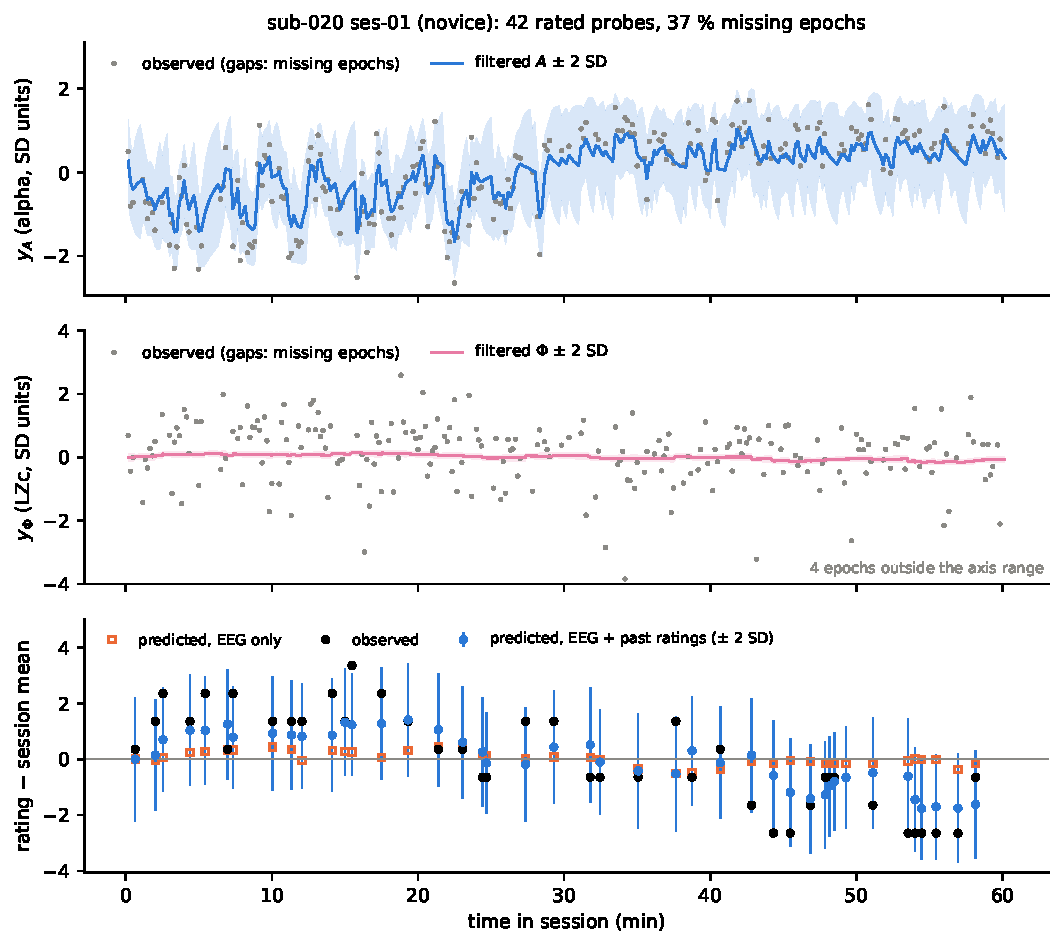
\includegraphics[width=0.49\textwidth]{fig9_realdata_session.pdf}\hfill
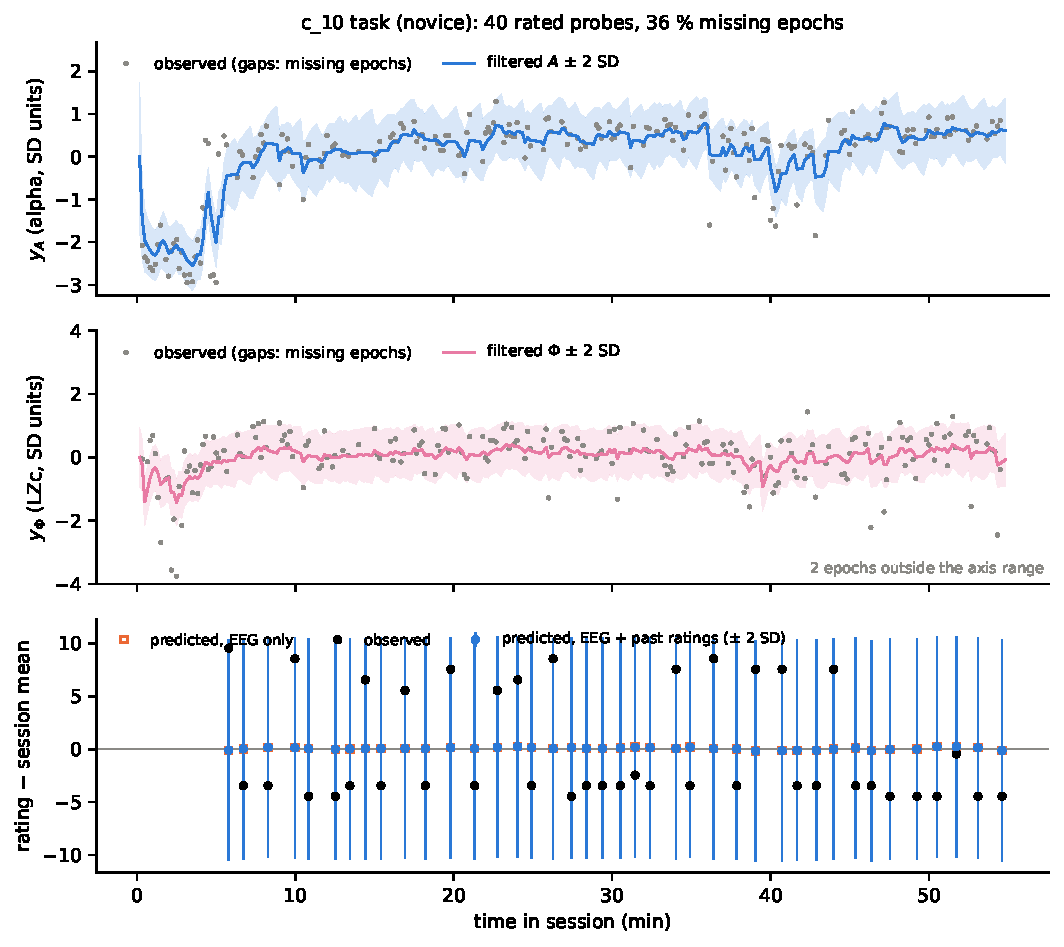
\includegraphics[width=0.49\textwidth]{fig11_osf_session.pdf}
\caption{\textbf{Một phiên được giữ của mỗi bộ dữ liệu, lọc bằng M1 tại ước lượng gộp (trong mẫu).} Trái: ds001787, sub-020 ses-01 (người mới); phải: OSF 3uszv, c\_10 (người mới); mỗi trường hợp là phiên được giữ có nhiều lần hỏi có điểm nhất. Trên: đại diện DMN $y_A$ và $A$ đã lọc $\pm2$ SD. Giữa: đại diện tích hợp $y_\Phi$ và $\Phi$ đã lọc $\pm2$ SD; trên ds001787 $\Phi$ đã lọc hầu như không động vì $y_\Phi$ gần như là nhiễu thuần, trên OSF 3uszv nó dao động theo thang vài chục giây; vài epoch ngoại lai nằm ngoài trục. Dưới: điểm tự chấm quy tâm trong phiên, với dự đoán một bước từ EEG và điểm quá khứ ($\pm2$ SD) và chỉ từ EEG. Khoảng trống là epoch thiếu. Trên OSF 3uszv đại diện alpha trôi theo thang phút, với các bước nhảy mức gần phút 5 và phút 40, và điểm luân phiên giữa khoảng $+7$ và $-5$ không có phụ thuộc chuỗi, nên mọi dự đoán nằm ở trung bình phiên.}
\label{fig:sessions}
\end{figure*}

\subsection{Sai số dự đoán và sai số đạt được (RQ1)}
Hình~\ref{fig:errors} là kết quả chính. Với bảy tham số không phụ thuộc thang của M1, nó cho thấy, trên mỗi bộ, CRB tính trước khi khoá, sai số chuẩn Fisher tại ước lượng, RMSE bootstrap và sai số chuẩn theo thông tin quan sát. Bảng~\ref{tab:errors} cho con số của hai hằng số tốc độ. Trên ds001787, cận của $\kinh$ tính trước khi xem bất kỳ EEG nào (9,1\,\%) và cận tính lại trên các phiên được giữ tại tỉ số tín hiệu trên nhiễu đo được (13,3\,\%) kẹp lấy 9,9\,\% đạt được, và bootstrap tái tạo giá trị Fisher (tỉ số 0,98). Trên OSF 3uszv, việc hỏi dày hơn và phiên dài hơn cho cận nhỏ hơn, 6,7\,\%, và sai số Fisher đạt được là 8,5\,\% với tỉ số bootstrap 1,03; tỉ số bootstrap trên Fisher là 0,98--1,69 trên ds001787 và 1,00--1,08 trên OSF 3uszv cho cả mười tham số, nên cổng E2 và F2 qua. Giả thuyết H1 được ủng hộ theo tiêu chí Fisher đã đăng ký trên cả hai bộ. Theo nghĩa Fisher, phân tích thiết kế chính xác trên ds001787 và hơi lạc quan trên OSF 3uszv, nơi sai số đạt được vượt cận tính lại trên các phiên được giữ 15\,\%; cả hai đều nằm gọn trong hệ số hai mà cận đã được kiểm chứng trên mô phỏng.

\begin{figure*}[t]
\centering
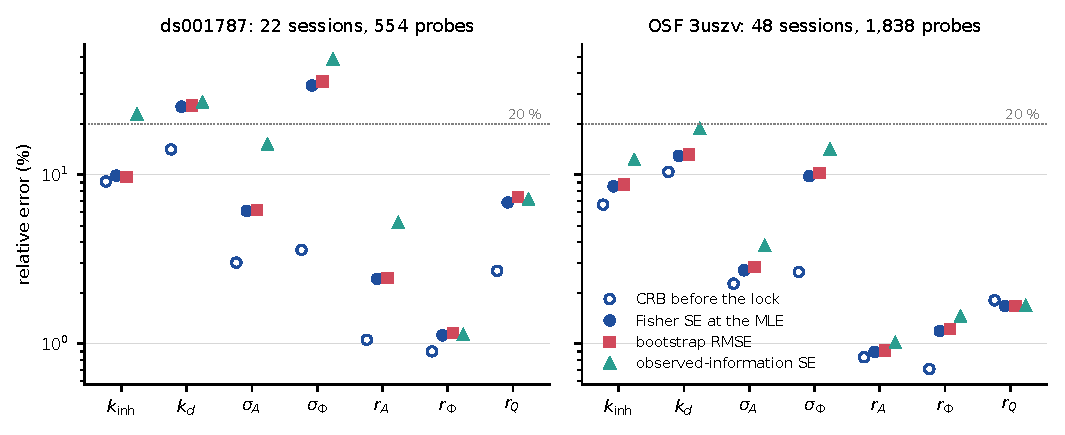
\includegraphics[width=0.95\textwidth]{fig1_pred_vs_achieved.pdf}
\caption{\textbf{Sai số tương đối dự đoán và đạt được của các tham số không phụ thuộc thang của M1 trên hai bộ dữ liệu.} Vòng tròn rỗng: cận Cramér--Rao từ thông tin Fisher chính xác tại tham số danh nghĩa trên lịch hỏi thật, tính trước mỗi lần khoá. Vòng tròn đặc: sai số chuẩn Fisher tại ước lượng hợp lý cực đại. Vuông: sai số căn quân phương của 200 lần fit lại bootstrap tham số. Tam giác: sai số chuẩn theo thông tin quan sát (Hessian số). Đường chấm là tiêu chí 20\,\% của giả thuyết H1. Với $\kinh$, ba con số đầu khớp nhau trên cả hai bộ (lớn nhất chia nhỏ nhất 1,08 và 1,32); với $\kd$, sai số Fisher vượt cận tính trước khi khoá 1,8 lần trên ds001787 và 1,2 lần trên OSF 3uszv; sai số theo thông tin quan sát của kênh công suất alpha ($\kinh$, $\sA$, $\rA$) vượt sai số Fisher 2,1--2,5 lần trên ds001787 và 1,1--1,4 lần trên OSF 3uszv.}
\label{fig:errors}
\end{figure*}

\begin{table}[t]
\caption{\textbf{Ba con số sai số cho hai hằng số tốc độ (phút$^{-1}$), là sai số tương đối tính bằng phần trăm.} CRB: trước khi khoá trên mọi thiết kế thật, trên các thiết kế được giữ, và trên các thiết kế đó với $\rA$ theo tỉ số tín hiệu trên nhiễu đo được. SE tại MLE: thông tin Fisher kỳ vọng, thông tin quan sát và hợp lý profile. RMSE: 200 lần fit lại bootstrap; tỉ số: RMSE chia SE Fisher (cổng E2/F2).}
\label{tab:errors}
\centering\scriptsize
\setlength{\tabcolsep}{2.2pt}
\begin{tabular}{llrrrrrrrrr}
\toprule
 & & & \multicolumn{3}{c}{CRB} & \multicolumn{3}{c}{SE tại MLE} & & \\
\cmidrule(lr){4-6}\cmidrule(lr){7-9}
Bộ dữ liệu & T.số & Ư.l. & khoá & giữ & SNR & Fisher & q.sát & prof. & RMSE & tỉ số \\
\midrule
ds001787  & $\kinh$ & 1,32  & 9,1  & 12,3 & 13,3 & 9,9  & 22,8 & 21,9 & 9,7  & 0,98 \\
          & $\kd$   & 0,200 & 14,1 & 19,0 & 19,1 & 25,3 & 26,7 & 26,6 & 25,7 & 1,01 \\
OSF 3uszv & $\kinh$ & 0,140 & 6,7  & 7,4  & 7,4  & 8,5  & 12,2 & 11,8 & 8,8  & 1,03 \\
          & $\kd$   & 1,58  & 10,4 & 11,5 & 11,5 & 12,9 & 18,7 & 18,3 & 13,2 & 1,02 \\
\bottomrule
\end{tabular}
\end{table}

\subsection{Dấu hiệu sai đặc tả (RQ1)}
Thông tin quan sát kể một câu chuyện khác cho kênh DMN. Trên ds001787, Hessian số cho 22,8\,\% với $\kinh$ và hợp lý profile cho 21,9\,\%, hơn gấp đôi giá trị Fisher; cùng hệ số đó, 2,1--2,5, xuất hiện với $\sA$ và $\rA$, trong khi với $\kd$, $\rPhi$ và $\rQ$ thông tin quan sát và kỳ vọng khớp nhau trong 6\,\%. Trên một bộ dữ liệu mô phỏng từ $\hat\thetav$ trên cùng 22 thiết kế, hệ số này cho $\kinh$, $\sA$ và $\rA$ là 1,05--1,07. Một khoảng cách khu trú ở một kênh và vắng mặt dưới mô hình đã fit là dấu hiệu sai đặc tả của kênh đó: công suất alpha vùng sau không được mô tả đầy đủ bởi một quá trình Ornstein--Uhlenbeck cộng nhiễu trắng. Trên OSF 3uszv dấu hiệu vẫn có nhưng yếu hơn, 1,43 với $\kinh$, 1,39 với $\sA$ và 1,13 với $\rA$ so với 0,93--0,99 trên dữ liệu mô phỏng, và không còn khu trú ở kênh alpha (1,45 với $\kd$, 1,44 với $\sPhi$); kiểm tra lặp lại R2, vốn đòi hệ số vượt 1,5, không đạt. Hình~\ref{fig:profiles} cho thấy các profile: trên ds001787 profile của $\kinh$ rộng khoảng gấp đôi đường bậc hai Fisher còn profile của $\kd$ bám theo nó; trên OSF 3uszv profile của $\kinh$ và $\kd$ rộng gấp 1,4 lần đường bậc hai, và profile của $\kappa$ bất đối xứng. Theo tiêu chí dựa trên hàm hợp lý, H1 vì thế không được ủng hộ trên ds001787 (21,9\,\%, vừa vượt 20\,\%) và được ủng hộ trên OSF 3uszv (11,8\,\%). Chúng tôi báo cáo khoảng profile làm độ bất định của $\kinh$ xuyên suốt.

\begin{figure*}[t]
\centering
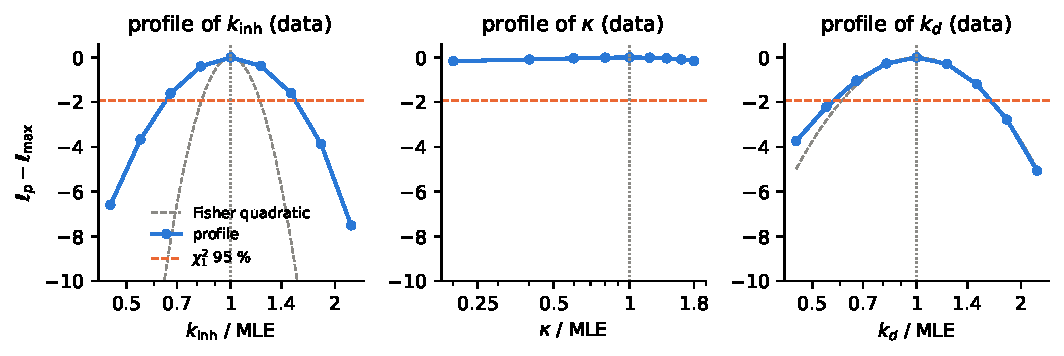
\includegraphics[width=0.82\textwidth]{fig10_realdata_profiles.pdf}\\[3pt]
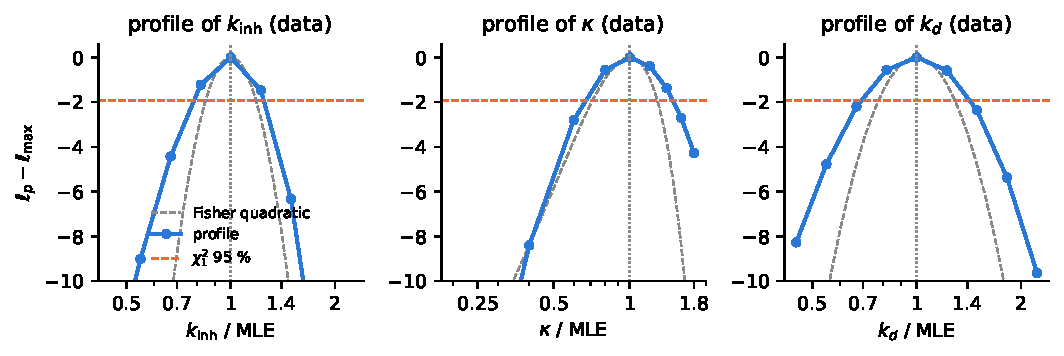
\includegraphics[width=0.82\textwidth]{fig12_osf_profiles.pdf}
\caption{\textbf{Log-hợp lý profile của ba hằng số tốc độ, mọi tham số khác được tối ưu lại tại mỗi điểm.} Trên: ds001787; dưới: OSF 3uszv. Nét đứt xám: xấp xỉ bậc hai suy từ thông tin Fisher kỳ vọng tại ước lượng hợp lý cực đại; cam: ngưỡng 95\,\% của $\chi^2_1$. Trên ds001787 profile của $\kinh$ rộng khoảng gấp đôi đường bậc hai (khoảng 95\,\% là 0,86--2,02~phút$^{-1}$), profile của $\kd$ bám theo nó, và profile của $\kappa$ phẳng vì $\hat\kappa\approx0$. Trên OSF 3uszv profile của $\kinh$ rộng gấp 1,38 lần đường bậc hai (0,110--0,175~phút$^{-1}$), của $\kd$ gấp 1,4 lần, và profile của $\kappa$, vốn âm, bất đối xứng (từ $-0{,}50$ đến $-0{,}23$).}
\label{fig:profiles}
\end{figure*}

\subsection{Ước lượng}
Bảng~\ref{tab:compare} đặt hai fit cạnh nhau. Trên ds001787 đại diện DMN hồi phục nhanh, $1/\hat k_{\mathrm{inh}}=0{,}76$~phút (khoảng profile 0,49--1,17~phút), so với 5~phút danh nghĩa của phân tích thiết kế, còn biến tích hợp ẩn chậm, $1/\hat k_d=5{,}0$~phút (3,1--8,7~phút); hệ số ghép $\kappa$ không phân biệt được với 0. Trên OSF 3uszv đại diện DMN chậm, $1/\hat k_{\mathrm{inh}}=7{,}1$~phút (5,7--9,1~phút), gấp chín lần giá trị của ds001787, còn biến tích hợp nhanh, $1/\hat k_d=0{,}63$~phút (0,45--0,91~phút), nhanh gấp tám lần trước: hai hằng số thời gian đã đổi chỗ cho nhau, và R1 trượt chín lần. Hệ số ghép nay xác định được và âm, $\hat\kappa=-0{,}33$ (từ $-0{,}50$ đến $-0{,}23$). Chất lượng các đại diện khác nhau giữa hai bộ. Trên ds001787 kênh DMN có tỉ số tín hiệu trên nhiễu 1,11 so với 1,58 danh nghĩa và kênh tích hợp 0,06 so với 2,4 danh nghĩa: thước đo độ phức tạp đã kiểm soát phổ hầu như không mang tín hiệu chậm. Trên OSF 3uszv kênh DMN đạt tỉ số danh nghĩa (1,57) và kênh tích hợp 0,54, gấp tám lần giá trị trên ds001787.

\begin{table*}[t]
\caption{\textbf{Hai fit đã đăng ký trước đặt cạnh nhau.} Hằng số thời gian tính bằng phút với khoảng profile 95\,\%; hệ số khuếch đại với khoảng Fisher 95\,\% và theo đơn vị SD trong phiên của điểm tự chấm (1,11 và 5,22). SE của $\kinh$: CRB trước khi khoá, Fisher, thông tin quan sát, hợp lý profile. Q.sát/kỳ vọng: SE theo thông tin quan sát chia SE theo thông tin kỳ vọng trên dữ liệu thật (trong ngoặc: trên dữ liệu mô phỏng từ fit). \mbox{\mathversion{normal}$\Delta$}LPD: mật độ dự đoán log ngoài mẫu của M1 trừ N2 (chỉ EEG) và trừ N1 (EEG và điểm quá khứ). Hiệu nhóm: $\log\kinh$, fit người lâu năm trừ fit người mới, khoảng Wald 95\,\%. Phân tích gộp: $1/\kinh$ hiệu ứng ngẫu nhiên trên những người có SE hữu hạn và SD giữa người $\tau$ của $\log\kinh$. Độ nhạy: số biến thể đã khoá giữ nguyên dấu của $\alpha$, dấu của $\beta$ và khoảng profile của $1/\kinh$.}
\label{tab:compare}
\centering\footnotesize
\setlength{\tabcolsep}{4pt}
\begin{tabular}{lll}
\toprule
 & ds001787 & OSF 3uszv \\
\midrule
Phiên giữ / ghi; số người                & 22 / 40; 16 & 48 / 58; 48 \\
Lần hỏi có điểm; khoảng hỏi; phiên      & 554; 1,6~phút; 45~phút & 1\,838; 77~s; 57~phút \\
Thang điểm; SD trong phiên               & $-3$ đến $3$; 1,11 & $-7$ đến $7$; 5,22 \\
$1/\kinh$ (phút)                         & 0,76 [0,49; 1,17] & 7,1 [5,7; 9,1] \\
$1/\kd$ (phút)                           & 5,0 [3,1; 8,7] & 0,63 [0,45; 0,91] \\
$\kappa$                                 & $\approx0$, profile phẳng & $-0{,}33$ [$-0{,}50$; $-0{,}23$] \\
SNR của $y_A$; của $y_\Phi$              & 1,11; 0,06 & 1,57; 0,54 \\
SE của $\kinh$: CRB / Fisher / q.\,sát / profile & 9,1 / 9,9 / 22,8 / 21,9\,\% & 6,7 / 8,5 / 12,2 / 11,8\,\% \\
RMSE bootstrap / SE Fisher của $\kinh$   & 0,98 & 1,03 \\
SE q.\,sát/kỳ vọng: $\kinh$, $\sA$, $\rA$ & 2,30; 2,48; 2,14 (1,05--1,07) & 1,43; 1,39; 1,13 (0,93--0,99) \\
$\alpha$ [95\,\%]; theo SD điểm          & 13,1 [4,9; 21,3]; 11,8 & 0,79 [$-0{,}24$; 1,82]; 0,15 \\
$\beta$ [95\,\%]; theo SD điểm           & $-0{,}03$ [$-0{,}19$; $0{,}13$]; $-0{,}02$ & 0,02 [$-0{,}34$; $0{,}38$]; 0,00 \\
$\Delta$LPD so với N2; so với N1         & $-0{,}010$; $-0{,}031$ & $+0{,}000$; $-0{,}001$ \\
Tự tương quan trễ 1 của điểm tự chấm     & 0,22 & $-0{,}01$ \\
Hiệu nhóm của $\log\kinh$                & $-1{,}19$ [$-1{,}56$; $-0{,}81$] & $+0{,}14$ [$-0{,}20$; $0{,}47$] \\
Phân tích gộp: $1/\kinh$; $\tau$; số người & 0,95 [0,40; 2,26]; 1,19; 9 & 3,3 [2,0; 5,7]; 1,49; 35 \\
Trung vị p Ljung--Box: $y_A$, $y_\Phi$   & 0,27; 0,40 & 0,06; 0,42 \\
Độ nhạy: $\alpha$, $\beta$, $1/\kinh$ giữ nguyên & 6/6; 4/6; 4/6 & 5/6; 1/6; 4/6 \\
Cổng                                     & E0--E3 qua & F0--F3 qua \\
\bottomrule
\end{tabular}
\end{table*}

\subsection{Hệ số khuếch đại và dự đoán ngoài mẫu (RQ2)}
Trên ds001787 hệ số khuếch đại từ biến tích hợp sang điểm là dương, $\hat\alpha=13{,}1$ (khoảng Fisher 95\,\% 4,9--21,3; không lần bootstrap nào ra giá trị không dương), như giả thuyết H3 dự đoán. Ý nghĩa của nó hạn chế: vì $y_\Phi$ thực chất là nhiễu, $\Phi$ ẩn được xác định hầu như hoàn toàn bởi chính điểm tự chấm, $\alpha$ và $\sPhi$ đánh đổi cho nhau (tương quan bootstrap giữa $\log\sPhi$ và $\alpha$: $-0{,}83$), và chỉ đóng góp của $\Phi$ vào phương sai điểm là xác định tốt. Trên OSF 3uszv, nơi $\Phi$ bị kênh độ phức tạp ghim lại, $\hat\alpha=0{,}79$ với khoảng chứa 0 (từ $-0{,}24$ đến $1{,}82$; 11 trong 200 lần bootstrap ra giá trị không dương): H3 không được ủng hộ. Theo đơn vị SD trong phiên của điểm, hệ số này là 11,8 trên ds001787 và 0,15 trên OSF 3uszv. Hệ số DMN là $\hat\beta=-0{,}03$ (từ $-0{,}19$ đến $0{,}13$) và $0{,}02$ (từ $-0{,}34$ đến $0{,}38$): dấu mà H4 hỏi không xác định được ở bộ nào, và công suất alpha vùng sau không đóng góp phát hiện được vào điểm.

Bảng~\ref{tab:loso} cho so sánh bỏ-một-phiên của giả thuyết H2. Trên ds001787, chỉ với EEG, M1 dự đoán điểm không tốt hơn hồi quy tức thời N2; với EEG và điểm quá khứ nó thắng trung bình chạy N3 nhưng không thắng mô hình chỉ có điểm N1, mô hình có mật độ dự đoán log tốt nhất và sai số nhỏ nhất trong mọi mô hình. Ưu thế so với N3 vì thế đến từ phụ thuộc chuỗi của báo cáo (tự tương quan trễ 1 là 0,22), không phải từ EEG. Trên OSF 3uszv, M1 không phân biệt được với N2 và N1 ($\Delta\mathrm{LPD}$ là $+0{,}0004$ và $-0{,}0006$), với sai số tuyệt đối trung bình 4,5--4,6 trên thang 14 mức cho mọi mô hình trừ trung bình chạy (4,7), và vì một lý do căn bản hơn: điểm của bộ này không có phụ thuộc chuỗi để mà dự đoán (tự tương quan trễ 1 là $-0{,}01$), nên điểm quá khứ cũng không giúp gì, và phân phối hai cực của chúng nằm ngoài tầm với của một hàm đọc ra Gauss (Phụ lục~\ref{app:ppc}). H2 không được ủng hộ ở bộ nào.

\begin{table*}[t]
\caption{\textbf{Dự đoán bỏ-một-phiên cho điểm tự chấm (giả thuyết H2), (a) chỉ từ EEG và (b) từ EEG và điểm quá khứ.} LPD: mật độ dự đoán log Gauss trung bình mỗi lần hỏi; MAE: sai số tuyệt đối trung bình. \mbox{\mathversion{normal}$\Delta$}LPD: M1 trừ mô hình rỗng với khoảng bootstrap 95\,\% theo phiên. N2: hồi quy tức thời lên $(y_A,y_\Phi)$; N1: M1 chỉ với kênh điểm; N3: trung bình chạy của điểm quá khứ.}
\label{tab:loso}
\centering\footnotesize
\setlength{\tabcolsep}{5pt}
\begin{tabular}{llrrrrr}
\toprule
 & So sánh & LPD M1 & LPD rỗng & $\Delta$LPD [95\,\%] & MAE M1 & MAE rỗng \\
\midrule
ds001787 & (a) với N2 & $-1{,}546$ & $-1{,}541$ & $-0{,}010$ [$-0{,}039$; $0{,}017$] & 0,93 & 0,92 \\
(554 lần hỏi) & (b) với N1 & $-1{,}472$ & $-1{,}421$ & $-0{,}031$ [$-0{,}103$; $0{,}009$] & 0,88 & 0,84 \\
 & (b) với N3 & $-1{,}472$ & $-1{,}626$ & $+0{,}154$ [$0{,}083$; $0{,}233$] & 0,88 & 1,00 \\
\midrule
OSF 3uszv & (a) với N2 & $-3{,}0746$ & $-3{,}0749$ & $+0{,}0004$ [$-0{,}0006$; $0{,}0014$] & 4,54 & 4,56 \\
(1\,838 lần hỏi) & (b) với N1 & $-3{,}0746$ & $-3{,}0740$ & $-0{,}0006$ [$-0{,}0018$; $0{,}0006$] & 4,54 & 4,55 \\
 & (b) với N3 & $-3{,}0746$ & $-3{,}1445$ & $+0{,}0712$ [$0{,}0609$; $0{,}0815$] & 4,54 & 4,66 \\
\bottomrule
\end{tabular}
\end{table*}

\subsection{Nhóm và từng người}
Trên ds001787, khi fit riêng, nhóm lâu năm có $\kinh$ nhỏ hơn nhóm mới (hiệu log $-1{,}19$, khoảng Wald 95\,\% từ $-1{,}56$ đến $-0{,}81$), ngược với giả thuyết H5. Hai fit riêng khác nhau chủ yếu ở cách chia phương sai công suất alpha giữa trạng thái và nhiễu quan sát (tỉ số tín hiệu trên nhiễu 1,05 so với 2,23), và $\kinh$ đánh đổi với cách chia đó: khi mọi tham số khác dùng chung, hiệu log co về $-0{,}18$ và kiểm định một bậc tự do đã đăng ký không có ý nghĩa ($\chi^2_1=3{,}3$, $p=0{,}068$), dù hai nhóm có khác nhau ở tham số nào đó ($\chi^2_{10}=41$). Hai nhóm còn khác nhau về giới và tuổi (10 trong 12 so với 2 trong 12 là nam, tuổi trung bình 39 so với 48). Trên OSF 3uszv, với 25 và 23 phiên, hai fit theo nhóm cho $\hat k_{\mathrm{inh}}=0{,}154$ và $0{,}134~\text{phút}^{-1}$, hiệu log $+0{,}14$ (từ $-0{,}20$ đến $0{,}47$; $\chi^2_1=2{,}67$, $p=0{,}10$), dưới khác biệt nhỏ nhất phát hiện được 0,37: cả F-H5a lẫn F-H5b đều không được ủng hộ, và hiệu thấy trên ds001787 không lặp lại. Hai nhóm khác nhau ở các tham số khác ($\chi^2_{10}=256$): ở người mới, biến tích hợp nhanh và ồn ($1/\kd=0{,}33$~phút, $\sPhi=1{,}1$) và gắn dương với báo cáo ($\alpha=2{,}0$, $\beta=+0{,}75$); ở người lâu năm nó chậm hơn ($1/\kd=0{,}89$~phút, $\sPhi=0{,}68$) và cả hai hệ số khuếch đại gần không hoặc âm ($\alpha=-0{,}15$, $\beta=-0{,}66$). Fit theo từng người cho sai số chuẩn hữu hạn ở 9 trong 16 người trên ds001787 và 35 trong 48 trên OSF 3uszv (ở phần lớn số còn lại $\sPhi$ được ước lượng bằng 0). Phân tích gộp của họ cho hằng số thời gian DMN 0,95~phút (0,40--2,26) và 3,3~phút (2,0--5,7) với độ lệch chuẩn giữa người của $\log\kinh$ là 1,19 và 1,49 đơn vị log ($I^2=0{,}92$ ở cả hai): các fit gộp cùng lắm mô tả một người tập trung bình.

\subsection{Kiểm tra mô hình và độ nhạy}
Innovation gần trắng trên ds001787 (trung vị p Ljung--Box $0{,}27$ cho $y_A$ và $0{,}40$ cho $y_\Phi$; bốn trong 22 phiên dưới 0,01 với $y_A$) và kém hơn trên OSF 3uszv ($p=0{,}058$ cho $y_A$, với 17 trong 48 phiên dưới 0,01; $0{,}42$ cho $y_\Phi$); innovation của hai kênh không tương quan ở cả hai (trung vị 0,05), nên ma trận nhiễu quan sát chéo được giữ. Kiểm tra dự đoán hậu nghiệm (Phụ lục~\ref{app:ppc}) tái tạo được phụ thuộc chuỗi của điểm trên ds001787 (tự tương quan trễ 1 là 0,22, mô phỏng 0,26, dải 0,15--0,37) và việc không có phụ thuộc chuỗi trên OSF 3uszv ($-0{,}01$; mô phỏng $-0{,}03$, dải từ $-0{,}08$ đến $0{,}02$), nhưng không tái tạo được phần giữa lệch của phân phối ds001787 lẫn phân phối hai cực của OSF, và trên cả hai bộ người lâu năm chấm điểm với độ phân tán nhỏ hơn mức mô hình gộp ngụ ý (OSF: hiệu SD trong phiên quan sát $-1{,}01$, mô phỏng $-0{,}31$, dải từ $-0{,}55$ đến $-0{,}05$).

Bảng~\ref{tab:sens} liệt kê các phân tích độ nhạy. Trên ds001787 $\alpha$ giữ dương ở cả sáu biến thể đã khoá, dấu của $\beta$ giữ ở bốn, và $1/\kinh$ nằm trong khoảng profile ở bốn: đại diện theta trán cho 4,0~phút, và biến thể chỉ giữ phiên có không quá 20\,\% epoch thiếu giữ hai phiên và suy biến. Trên OSF 3uszv biến thể đó không giữ phiên nào, vì riêng cửa sổ hỏi đã vượt 20\,\% ở mọi phiên, một sơ suất của bản đăng ký, nên sáu biến thể chạy được; dấu của $\alpha$ giữ ở năm (nó âm với đại diện số mũ aperiodic), dấu của $\beta$ ở một, và $1/\kinh$ nằm trong khoảng ở bốn (theta trán cho 17~phút và z-score theo phiên 4,8~phút). Quy tắc 80\,\% vì thế đạt với dấu của $\alpha$ trên cả hai bộ và không với gì khác, và các ước lượng được trình bày theo lối mô tả. Một biến thể ngoài đăng ký trên OSF 3uszv, thêm sau khi xem Hình~\ref{fig:sessions}, che EEG trước lần hỏi đầu tiên (các phiên mở đầu bằng hướng dẫn và một lần hỏi tập dượt, tiếng chuông đầu tiên đến sau trung bình 6,8~phút): hằng số thời gian DMN tăng từ 7,1 lên 16~phút, nên bước chuyển mức alpha ở đầu phiên là phần nhanh nhất của đại diện này.

\begin{table*}[t]
\caption{\textbf{Phân tích độ nhạy: ước lượng gộp, hằng số thời gian tính bằng phút.} Quy tắc cố định 150~$\mu$V là quy tắc chính đã khoá của ds001787 và một biến thể đã khoá của OSF 3uszv; quy tắc thích ứng là biến thể ngoài đăng ký của ds001787 và quy tắc chính đã khoá của OSF 3uszv. Dòng cuối là biến thể ngoài đăng ký và không tính vào quy tắc độ bền. Trên ds001787 biến thể không quá 20\,\% epoch thiếu giữ hai phiên và suy biến; trên OSF 3uszv nó không giữ phiên nào.}
\label{tab:sens}
\centering\footnotesize
\setlength{\tabcolsep}{5pt}
\begin{tabular}{lrrrrrrrr}
\toprule
 & \multicolumn{4}{c}{ds001787} & \multicolumn{4}{c}{OSF 3uszv} \\
\cmidrule(lr){2-5}\cmidrule(lr){6-9}
Biến thể & $n$ & $\alpha$ & $\beta$ & $1/\kinh$ & $n$ & $\alpha$ & $\beta$ & $1/\kinh$ \\
\midrule
Phân tích chính                      & 22 & 13,10 & $-0{,}026$ & 0,76 & 48 & 0,79 & $+0{,}018$ & 7,12 \\
$y_A$: alpha tuần hoàn               & 22 & 13,10 & $-0{,}069$ & 0,52 & 48 & 0,79 & $+0{,}069$ & 7,74 \\
$y_A$: theta trán                    & 22 & 13,08 & $-0{,}389$ & 3,98 & 48 & 0,76 & $-0{,}293$ & 16,76 \\
$y_\Phi$: số mũ aperiodic đổi dấu    & 22 & 13,08 & $+0{,}045$ & 0,76 & 48 & $-0{,}10$ & $-0{,}127$ & 7,91 \\
z-score theo phiên                   & 22 & 13,10 & $-0{,}051$ & 0,90 & 48 & 0,82 & $-0{,}108$ & 4,81 \\
Không quá 20\,\% epoch thiếu         &  2 & 399,6 & $-0{,}239$ & 0,23 &  0 & -- & -- & -- \\
20 lần hỏi đầu                       & 22 & 13,09 & $+0{,}096$ & 0,76 & 48 & 1,43 & $-0{,}096$ & 7,10 \\
Quy tắc cố định 150~$\mu$V           & \multicolumn{4}{c}{(chính)} & 24 & 0,36 & $-0{,}470$ & 5,74 \\
Quy tắc thích ứng                    & 39 & 0,97 & $+0{,}215$ & 0,48 & \multicolumn{4}{c}{(chính)} \\
Che EEG trước lần hỏi đầu            & -- & -- & -- & -- & 48 & 1,02 & $+0{,}285$ & 16,00 \\
\bottomrule
\end{tabular}
\end{table*}

\subsection{So sánh với tham số của BQI (RQ3)}
\label{sec:res-bqi}
Bảng~\ref{tab:bqi} đặt các ước lượng cạnh các dự đoán T1--T5 của BQI (Mục~\ref{sec:theory-pred}) và các giá trị mà BQI fit từ dữ liệu phân tích gộp \cite[Bảng~5]{BQI}. Hằng số thời gian không phụ thuộc thang nên so trực tiếp được; hệ số ghép và các hệ số khuếch đại phụ thuộc đơn vị của các đại diện đã chuẩn hoá và của thang điểm, nên chỉ so được dấu. Không bộ nào tái tạo được các hằng số thời gian của BQI: hằng số thời gian DMN là 0,76 và 7,1~phút so với 23~phút, hằng số thời gian tích hợp là 5,0 và 0,63~phút so với 29~phút, và giá trị BQI nằm ngoài cả bốn khoảng profile. Hệ số ghép, dương trong \cite[pt.~(53)]{BQI}, không phân biệt được với 0 trên ds001787 và âm trên OSF 3uszv. Hệ số $\alpha$ dương ở cả hai bộ như trong BQI, nhưng khoảng tin cậy chỉ loại 0 trên ds001787; dấu của $\beta$, dương trong BQI, không xác định được ở bộ nào; và khác biệt nhóm suy ra từ \cite[pt.~(51) và Mục~7.5]{BQI} bị đảo chiều trên ds001787 và vắng mặt trên OSF 3uszv. Trong năm dự đoán, chỉ T3 được tái tạo về dấu, và chỉ xác định được dấu trên ds001787.

\begin{table*}[t]
\caption{\textbf{Giá trị tham số của BQI và các ước lượng trên hai bộ dữ liệu.} BQI: fit bình phương tối thiểu từ dữ liệu phân tích gộp \cite[Bảng~5]{BQI}. Hằng số thời gian tính bằng phút với khoảng profile 95\,\%; $\kappa$ với khoảng profile; hệ số khuếch đại với khoảng Fisher 95\,\%; hiệu nhóm của $\log\kinh$ (lâu năm trừ mới) với khoảng Wald. Hệ số ghép và hệ số khuếch đại tính theo đơn vị của các đại diện và điểm đã chuẩn hoá, nên chỉ so được dấu với BQI.}
\label{tab:bqi}
\centering\footnotesize
\setlength{\tabcolsep}{5pt}
\begin{tabular}{llll}
\toprule
Đại lượng & BQI & ds001787 & OSF 3uszv \\
\midrule
$1/\kinh$ (phút) & 23 & 0,76 [0,49; 1,17] & 7,1 [5,7; 9,1] \\
$1/\kd$ (phút) & 29 & 5,0 [3,1; 8,7] & 0,63 [0,45; 0,91] \\
Dấu của $\kappa$ & $+$ & $\approx0$, profile phẳng & $-$ ($-0{,}33$ [$-0{,}50$; $-0{,}23$]) \\
Dấu của $\alpha$ & $+$ (2,34) & $+$ (13,1 [4,9; 21,3]) & $+$, chưa xác định (0,79 [$-0{,}24$; 1,82]) \\
Dấu của $\beta$ & $+$ (1,87) & chưa xác định & chưa xác định \\
Lâu năm $-$ mới, $\log\kinh$ & $>0$ & $-1{,}19$ [$-1{,}56$; $-0{,}81$] & $+0{,}14$ [$-0{,}20$; 0,47] \\
\bottomrule
\end{tabular}
\end{table*}

\subsection{Điều gì lặp lại (RQ4)}
Bảng~\ref{tab:tests} liệt kê mọi giả thuyết và kiểm tra đã đăng ký cùng kết cục. Ba kết quả chung cho hai bộ và hai kết quả thì không. (i) Các con số sai số theo Fisher chính xác trên cả hai: với $\kinh$, cận tính trước khi khoá, SE Fisher tại ước lượng và RMSE bootstrap chênh nhau nhiều nhất 8\,\% trên ds001787 và 32\,\% trên OSF 3uszv, và trên cả hai SE dựa trên hàm hợp lý của kênh alpha vượt SE Fisher. (ii) Không đại diện EEG nào cải thiện dự đoán ngoài mẫu cho báo cáo ở bộ nào. (iii) Độ dị biệt giữa người của $\log\kinh$ lớn ở cả hai ($\tau$ là 1,2 và 1,5). (iv) $\alpha>0$ không lặp lại: ước lượng dương ở cả hai, nhưng khoảng tin cậy chỉ loại 0 trên ds001787, và ở cả hai giá trị của nó theo SD của điểm nói lên ít điều. (v) Bản thân các hằng số tốc độ không lặp lại: $1/\kinh$ là 0,76~phút trên ds001787 và 7,1~phút trên OSF 3uszv, $1/\kd$ là 5,0 so với 0,63~phút, và chiều của khác biệt nhóm khác nhau.

\begin{table*}[t]
\caption{\textbf{Các giả thuyết đã đăng ký và kiểm tra lặp lại cùng kết cục trên hai bộ dữ liệu (khoảng là 95\,\%).}}
\label{tab:tests}
\centering\scriptsize
\setlength{\tabcolsep}{3pt}
\begin{tabular}{lll}
\toprule
Giả thuyết & ds001787 & OSF 3uszv \\
\midrule
H1: SE của $\kinh$ không quá 20\,\% & Fisher 9,9\,\% (profile 21,9\,\%): ủng hộ (Fisher) & Fisher 8,5\,\% (profile 11,8\,\%): ủng hộ \\
H2: M1 thắng các mô hình rỗng & $\Delta$LPD $-0{,}010$ (N2), $-0{,}031$ (N1): không ủng hộ & $+0{,}0004$ (N2), $-0{,}0006$ (N1): không ủng hộ \\
H3: $\alpha>0$ & 13,1 [4,9; 21,3]: ủng hộ & 0,79 [$-0{,}24$; 1,82]: không ủng hộ \\
H4: dấu của $\beta$ & $-0{,}03$ [$-0{,}19$; 0,13]: không xác định & 0,02 [$-0{,}34$; 0,38]: không xác định \\
H5: $\kinh$ cao hơn ở người lâu năm & $-1{,}19$ [$-1{,}56$; $-0{,}81$]; LR $p=0{,}068$: không ủng hộ & $+0{,}14$ [$-0{,}20$; 0,47]; LR $p=0{,}10$: không ủng hộ (a, b) \\
R1: $1/\kinh$ trong 0,49--1,17 phút & -- & 7,1 phút [5,7; 9,1]: không lặp lại \\
R2: SE q.sát/kỳ vọng $>1{,}5$, $\approx1$ khi mô phỏng & 2,30; 1,05 & 1,43; 0,93: không lặp lại \\
R3: $1/\kd$ & 5,0 phút [3,1; 8,7] & 0,63 phút [0,45; 0,91] \\
\bottomrule
\end{tabular}
\end{table*}

\subsection{Vì sao hằng số thời gian khác nhau: một mô phỏng}
Việc hai hằng số thời gian đổi chỗ có một cách đọc đơn giản. Trên ds001787, đại diện độ phức tạp là nhiễu, nên $\Phi$ và $\kd$ được xác định bởi điểm tự chấm và $1/\kd$ đo sự trôi chậm của báo cáo; trên OSF 3uszv đại diện độ phức tạp mang tín hiệu 40~s ghim $\Phi$ lại, báo cáo không trôi, còn đại diện alpha trôi theo thang phút trong các phiên dài một giờ (Hình~\ref{fig:sessions}). Hình~\ref{fig:sim} cho thấy fit Ornstein--Uhlenbeck làm gì với một đặc trưng như vậy. Khi đặc trưng là tổng của một thành phần nhanh (0,5~phút) và một thành phần chậm (3, 7 hoặc 15~phút), hằng số thời gian fit được dịch đơn điệu từ giá trị nhanh sang giá trị chậm khi tỉ trọng phương sai của thành phần chậm tăng: với tỉ trọng bằng nhau fit trả về 1,2; 1,7 và 1,9~phút, và giá trị chậm chỉ đạt được khi thành phần chậm chiếm gần hết phương sai (ở tỉ trọng 0,8, thành phần 7~phút cho 3,6~phút và thành phần 15~phút cho 7,5~phút). Một hằng số tốc độ duy nhất ước lượng từ một đặc trưng chưa hiệu chuẩn vì thế là tổng hợp có trọng số phương sai của mọi thang thời gian mà đặc trưng đó chứa trong bản ghi đó, phụ thuộc vào montage, độ dài phiên và phương pháp tập; đại diện theta trán cho 4~phút trên bộ này và 17~phút trên bộ kia cũng vì lý do đó. Hằng số thời gian DMN của M1 là tính chất của đặc trưng, chưa phải của một quá trình DMN.

\begin{figure}[t]
\centering
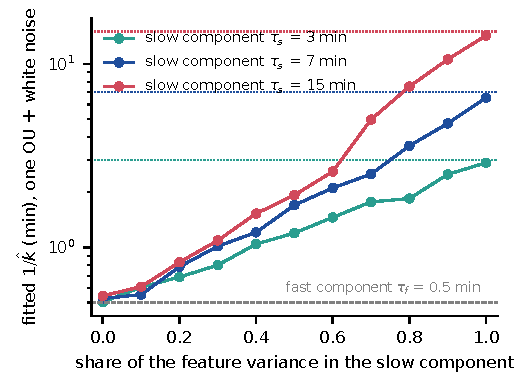
\includegraphics[width=\columnwidth]{fig2_ou_timescale.pdf}
\caption{\textbf{Fit Ornstein--Uhlenbeck trả về thang thời gian trội của đặc trưng được đưa vào.} Đặc trưng mô phỏng là tổng của một thành phần nhanh ($\tau_f=0{,}5$~phút), một thành phần chậm ($\tau_s$ bằng 3, 7 hoặc 15~phút, đường chấm) và nhiễu trắng, trên thiết kế của OSF 3uszv (48 phiên 57~phút với cửa sổ hỏi và thêm 10\,\% epoch thiếu). Nó được fit bằng một quá trình Ornstein--Uhlenbeck cộng nhiễu trắng, tức kênh DMN của M1. Hằng số thời gian fit được dịch từ $\tau_f$ sang $\tau_s$ khi tỉ trọng phương sai của thành phần chậm tăng.}
\label{fig:sim}
\end{figure}
